%!TEX root = ../dissertation.tex

\chapter{Solution}
\label{chapter:solution}
Usually, provisioning the components of a smart place application is an operation
that is manually executed and requires expertise since that the software components must
be correctly installed and configured. Furthermore, every time that a new smart place is deployed
these operations must be repeated. With that in mind, in order to make the deployment of
smart places more efficient in Section~\ref{sec:sol_provisioning} we propose a solution
that automates the provision of smart places application in the cloud.\\

In the present work our main goal is to determine if a cloud-based deployment can meet the
requirements of RFID-based smart place applications, as mentioned in Section~\ref{section:objectives}.
To achieve our goals we will follow two approaches to deploy the smart warehouse application: cloud
and fog. In Section~\ref{sec:sol_smart_warehouse_deployment}, we describe the alternative
architectures of the smart warehouse deployment.\\

% Provisioning
\section{Smart Place Provisioning}
\label{sec:sol_provisioning}
In this section we propose a mechanism that automates the provisioning of software for smart place
applications in the cloud. Our solution relies on \acrfull{CM} tools that leverage
existing software stacks. Figure~\ref{fig:provisioning_generic_architecture} presents the architecture
for the proposed mechanism.\\

% Provisioning mechanism conceptual architecture
\begin{figure}[ht!]
\centering
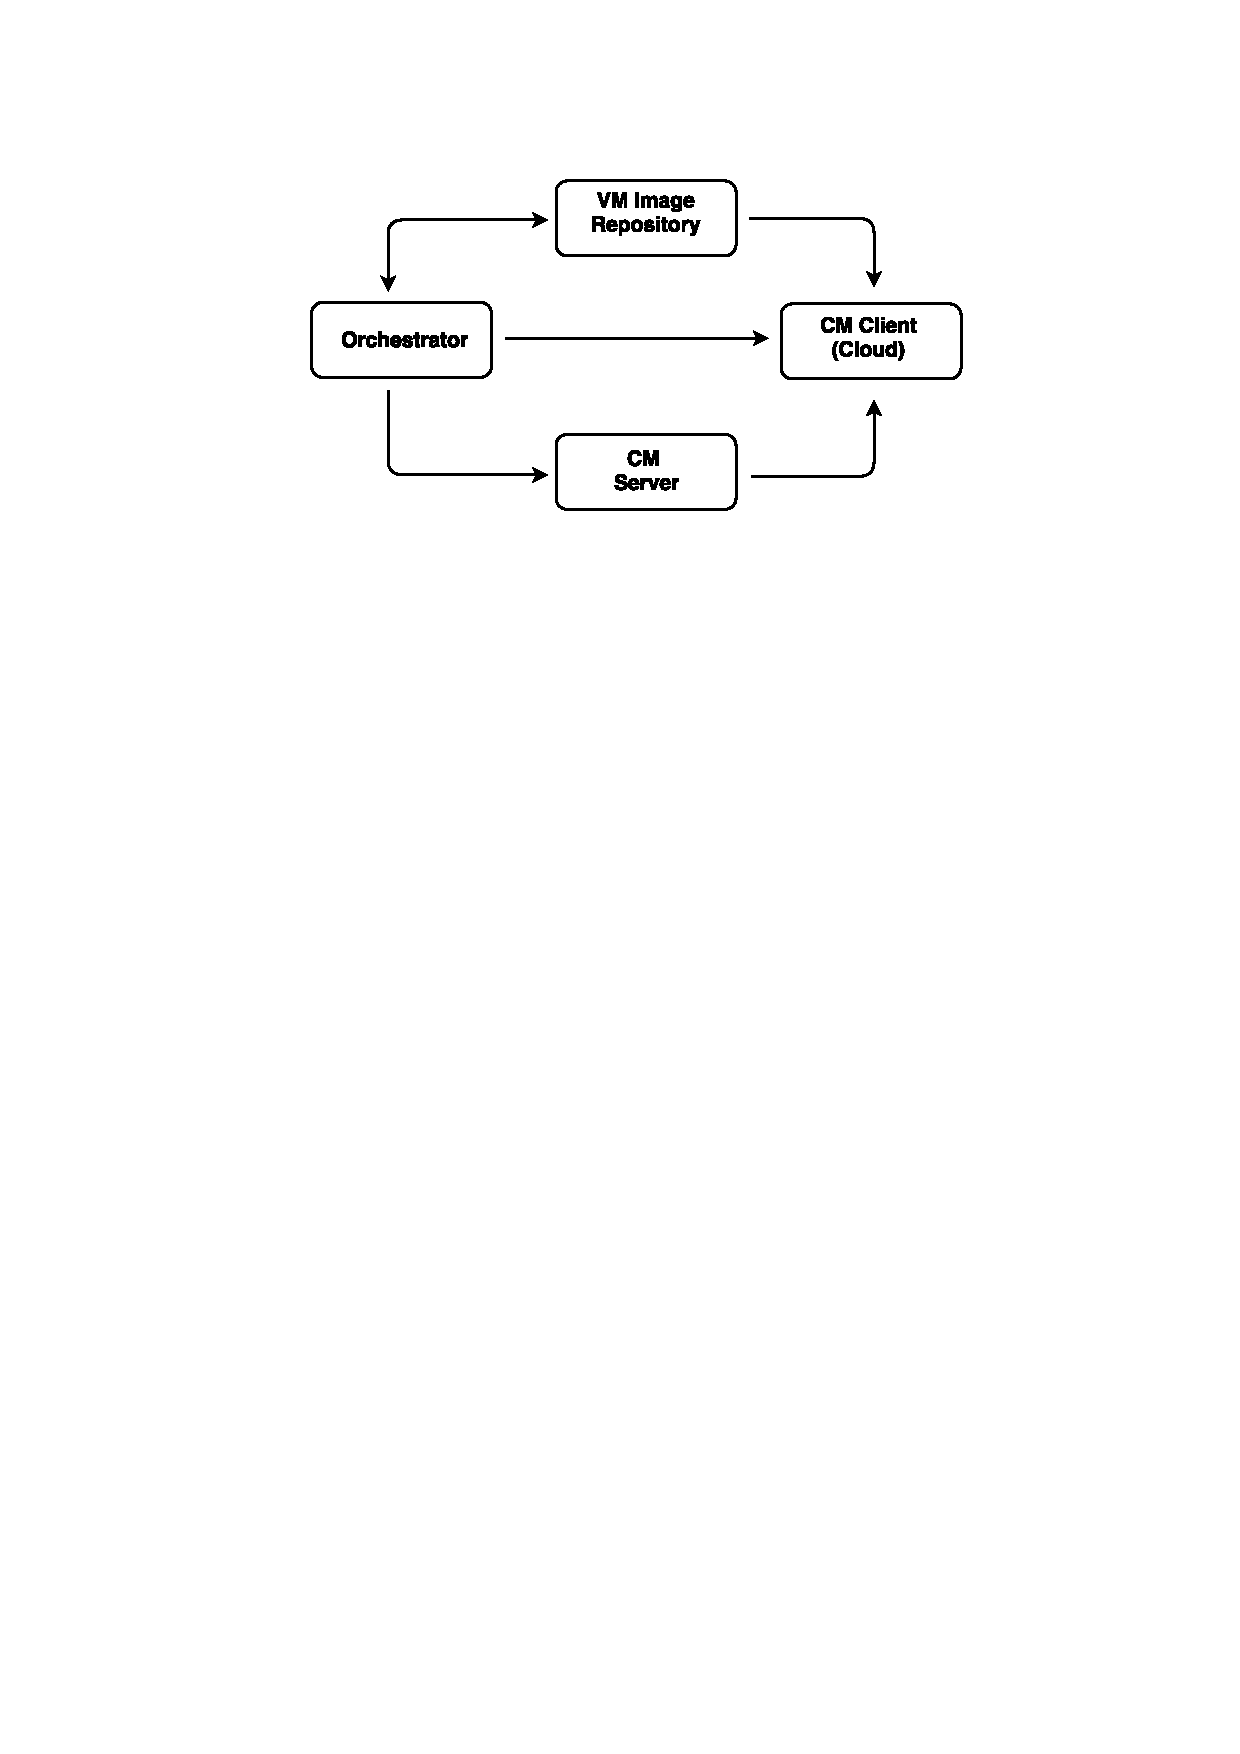
\includegraphics[width=.7\textwidth]{images/c4t-generic-solution.pdf}
\caption[Provisioning mechanism conceptual architecture.]{Provisioning mechanism conceptual architecture.}
\label{fig:provisioning_generic_architecture}
\end{figure}

In the proposed architecture, the provisioning of a smart place is based on provisioning policies and
software images that are defined and configured in a development environment. The provisioning policies
allow to define which components of software must be provisioned in a given instance, configure
management tasks such as to trigger a notification when a resource state changes. The software images
contains all the software components required to deploy the application.\\

After the provisioning policies were defined and configured, the Orchestrator uploads them to its respective
remote repositories (CM Server and VM Image Repository). When the provisioning request is performed -
through a configuration management interface provided by the Orchestrator - the configuration management
client (\gls{CM} Client) in the cloud server pulls the polices from the configuration management server
(\gls{CM} Server), a centralized server that is responsible to maintain a consistent state of the
provisioned nodes in the cloud. In order to enforce the polices, the \gls{CM} Client pulls the software
images from a central repository and then performs the provisioning and configuration of the software.
After provisioning the infrastructure, the CM client periodically polls the CM server in order to
determine if its current state is consistent with the most recent policy.

% Implementation Details
\subsection{Implementation Details}
\label{sub:Implementation Details}
The implementation of the provisioning mechanism relies on the Chef tool. Chef provides several features
that allow to describe our infrastructure as code. In the implementation of the provisioning mechanism,
the main features used were the Chef \textit{recipes}, \textit{roles} and \textit{knife} command-line
tool\footnote{The tool uses culinary analogy in most of its concepts}. In the current implementation,
we used Docker containers to provisioning the smart warehouse software at the cloud providers in
alternative to traditional \glspl{VM}.

% Provisioning Recipes
\subsubsection{Provisioning Recipes}
\label{subs:recipes}
The \textit{recipes} that describe our infrastructure are based on \textit{cookbooks} available at the
Chef Supermarket\footnote{\url{https://supermarket.chef.io/}} and also in custom recipes that
were defined specifically for this work to describe how the Fosstrak software stack is provisioned
in the cloud. Since we are using Docker containers the recipes were defined based on the official
Docker cookbook for describing how the containers must be provisioned. For instance, Listing~\ref{listing:epcis_recipe}
present the provisioning recipe for the Docker container that runs the \gls{EPCIS} Repository:

% EPCIS container recipe
\begin{listing}
\inputminted[frame=lines,
             framesep=3mm,
             linenos=true,
             xleftmargin=21pt,
             tabsize=4]{ruby}{./listings/epcis_recipe.rb}
\caption{EPCIS Docker container provisioning recipe.}
\label{listing:epcis_recipe}
\end{listing}

The recipe specification describes that first the Docker image \textit{cloud4things$/$fosstrak-epcis}
must be pulled from the central repository. In particular, this image contains the software required
to deploy the \gls{EPCIS} repository web application, namely an Apache Tomcat web-server and the \gls{EPCIS}
repository source code. Finally, the recipe describes that the image \textit{cloud4things$/$fosstrak-epcis}
must be used to create a container named \textit{fosstrak-epcis} and the port \textit{8080} need to
be exposed. Furthermore this container must be linked to the container \textit{fosstrak-db} that
internally is represented by the alias \textit{db}. The \textit{detach} parameter describes if the
container must run in the background or not.\\

We also defined the recipes that provision Docker containers for the remaining Fosstrak
stack, namely the \textit{Filtering \& Collection Server} (Listing~\ref{listing:ale_recipe}),
\textit{Capturing Application} (Listing~\ref{listing:capture_recipe}) and \textit{MySQL}
database (Listing~\ref{listing:db_recipe}).

% ALE container recipe
\begin{listing}
\inputminted[frame=lines,
             framesep=3mm,
             linenos=true,
             xleftmargin=21pt,
             tabsize=4]{ruby}{./listings/ale_recipe.rb}
\caption{ALE Docker container provisioning recipe.}
\label{listing:ale_recipe}
\end{listing}

% Capturing app container recipe
\begin{listing}
\inputminted[frame=lines,
             framesep=3mm,
             linenos=true,
             xleftmargin=21pt,
             tabsize=4]{ruby}{./listings/capture_recipe.rb}
\caption{Capturing application Docker container provisioning recipe.}
\label{listing:capture_recipe}
\end{listing}

% Database container recipe
\begin{listing}
\inputminted[frame=lines,
             framesep=3mm,
             linenos=true,
             xleftmargin=21pt,
             tabsize=4]{ruby}{./listings/db_recipe.rb}
\caption{MySQL Docker container provisioning recipe.}
\label{listing:db_recipe}
\end{listing}

% Provisioning Roles
\subsubsection{Provisioning Roles}
\label{subs:provisioning_roles}
A \textit{role} is a categorization that describes what are the responsibilities of a specific
node, what settings and software components should be given to it. For instance, it is possible
to define what are the nodes that includes the database, web server, etc. The roles allows to describe
the smart place application topology in the cloud.\\

The roles that describe the smart warehouse application topology were defined based in the
technological architecture of the smart warehouse for the cloud and fog concepts, presented in Section~\ref{sec:impl_smart_place}.
In the next sections, we describe with more detail the roles that were defined to provisioning the
smart place infrastructure.

% Cloud Provisioning Roles
\subparagraph{Cloud Provisioning Roles.}
\label{subp:cloud_roles}
In a cloud deployment approach the Fosstrak software stack is provisioned in a single instance, as
illustrated in Figure~\ref{fig:implementation_cloud_architecture}. Thus, we defined a single role
to describe the responsibilities of the node provisioned in the cloud.\\

% Fosstrak role
\begin{listing}[ht!]
\inputminted[frame=lines,
             framesep=3mm,
             linenos=true,
             xleftmargin=21pt,
             tabsize=4]{json}{./listings/fosstrak_role.json}
\caption{Cloud Deployment: provisioning role.}
\label{listing:cloud_recipe}
\end{listing}

The \textit{fosstrak} role describes that the nodes must have installed all the modules of Fosstrak
that are specified in the docker \textit{cookbook}: \textit{docker}, \textit{fosstrak-db},
\textit{fosstrak-epcis}, \textit{fosstrak-capture} and \textit{fosstrak-ale} recipes. The nodes
that have assigned this role are identified as \textit{fosstrak-server}.

% Fog Provisioning Roles
\subparagraph{Fog Provisioning Roles.}
\label{subp:fog_roles}
In a fog deployment approach the Fosstrak software stack is distributed across the fog and cloud,
as illustrated on Figure~\ref{fig:implementation_fog_architecture}. Therefore, we defined two different
roles that describe the responsibilities of the provisioned nodes.

% Fog role
\begin{listing}[ht!]
\inputminted[frame=lines,
             framesep=3mm,
             linenos=true,
             xleftmargin=21pt,
             tabsize=4]{json}{./listings/fog_role.json}
\caption{Fog Deployment: Fog provisioning role.}
\label{listing:fog_fog_recipe}
\end{listing}

The \textit{fog} role describes that fog nodes must have installed the following resources specified in the
recipes of the docker \textit{cookbook}: \textit{docker}, \textit{fosstrak-capture} and
\textit{fosstrak-ale}. The nodes that have assigned this role are identified as \textit{fog-server},
as illustrated in Listing~\ref{listing:fog_fog_recipe}.\\

% Cloud role
\begin{listing}[ht!]
\inputminted[frame=lines,
             framesep=3mm,
             linenos=true,
             xleftmargin=21pt,
             tabsize=4]{json}{./listings/cloud_role.json}
\caption{Fog deployment: Cloud provisioning role.}
\label{listing:fog_cloud_recipe}
\end{listing}

The \textit{cloud} role describes that cloud nodes must have installed the remaining modules of Fosstrak
that are specified in the docker \textit{cookbook}: \textit{docker}, \textit{fosstrak-db} and
\textit{fosstrak-epcis} recipes. The nodes that have assigned this role are identified as
\textit{cloud-server}, as illustrated in Listing~\ref{listing:fog_cloud_recipe}.

% Provisioning Mechanism
\subsubsection{Provisioning Mechanism}
\label{subs:provisioning_mechanism}
To provisioning the resources in the cloud instances we used \textit{knife}, a command-line tool
developed by Chef that provides an interface between the local Chef repository and the Chef server.
The provisioning workflow is illustrated in Figure~\ref{fig:provisioning_tech_architecture}.\\

% Automatic provisioning diagram
\begin{figure}[ht!]
\centering
\makebox[\textwidth][c]{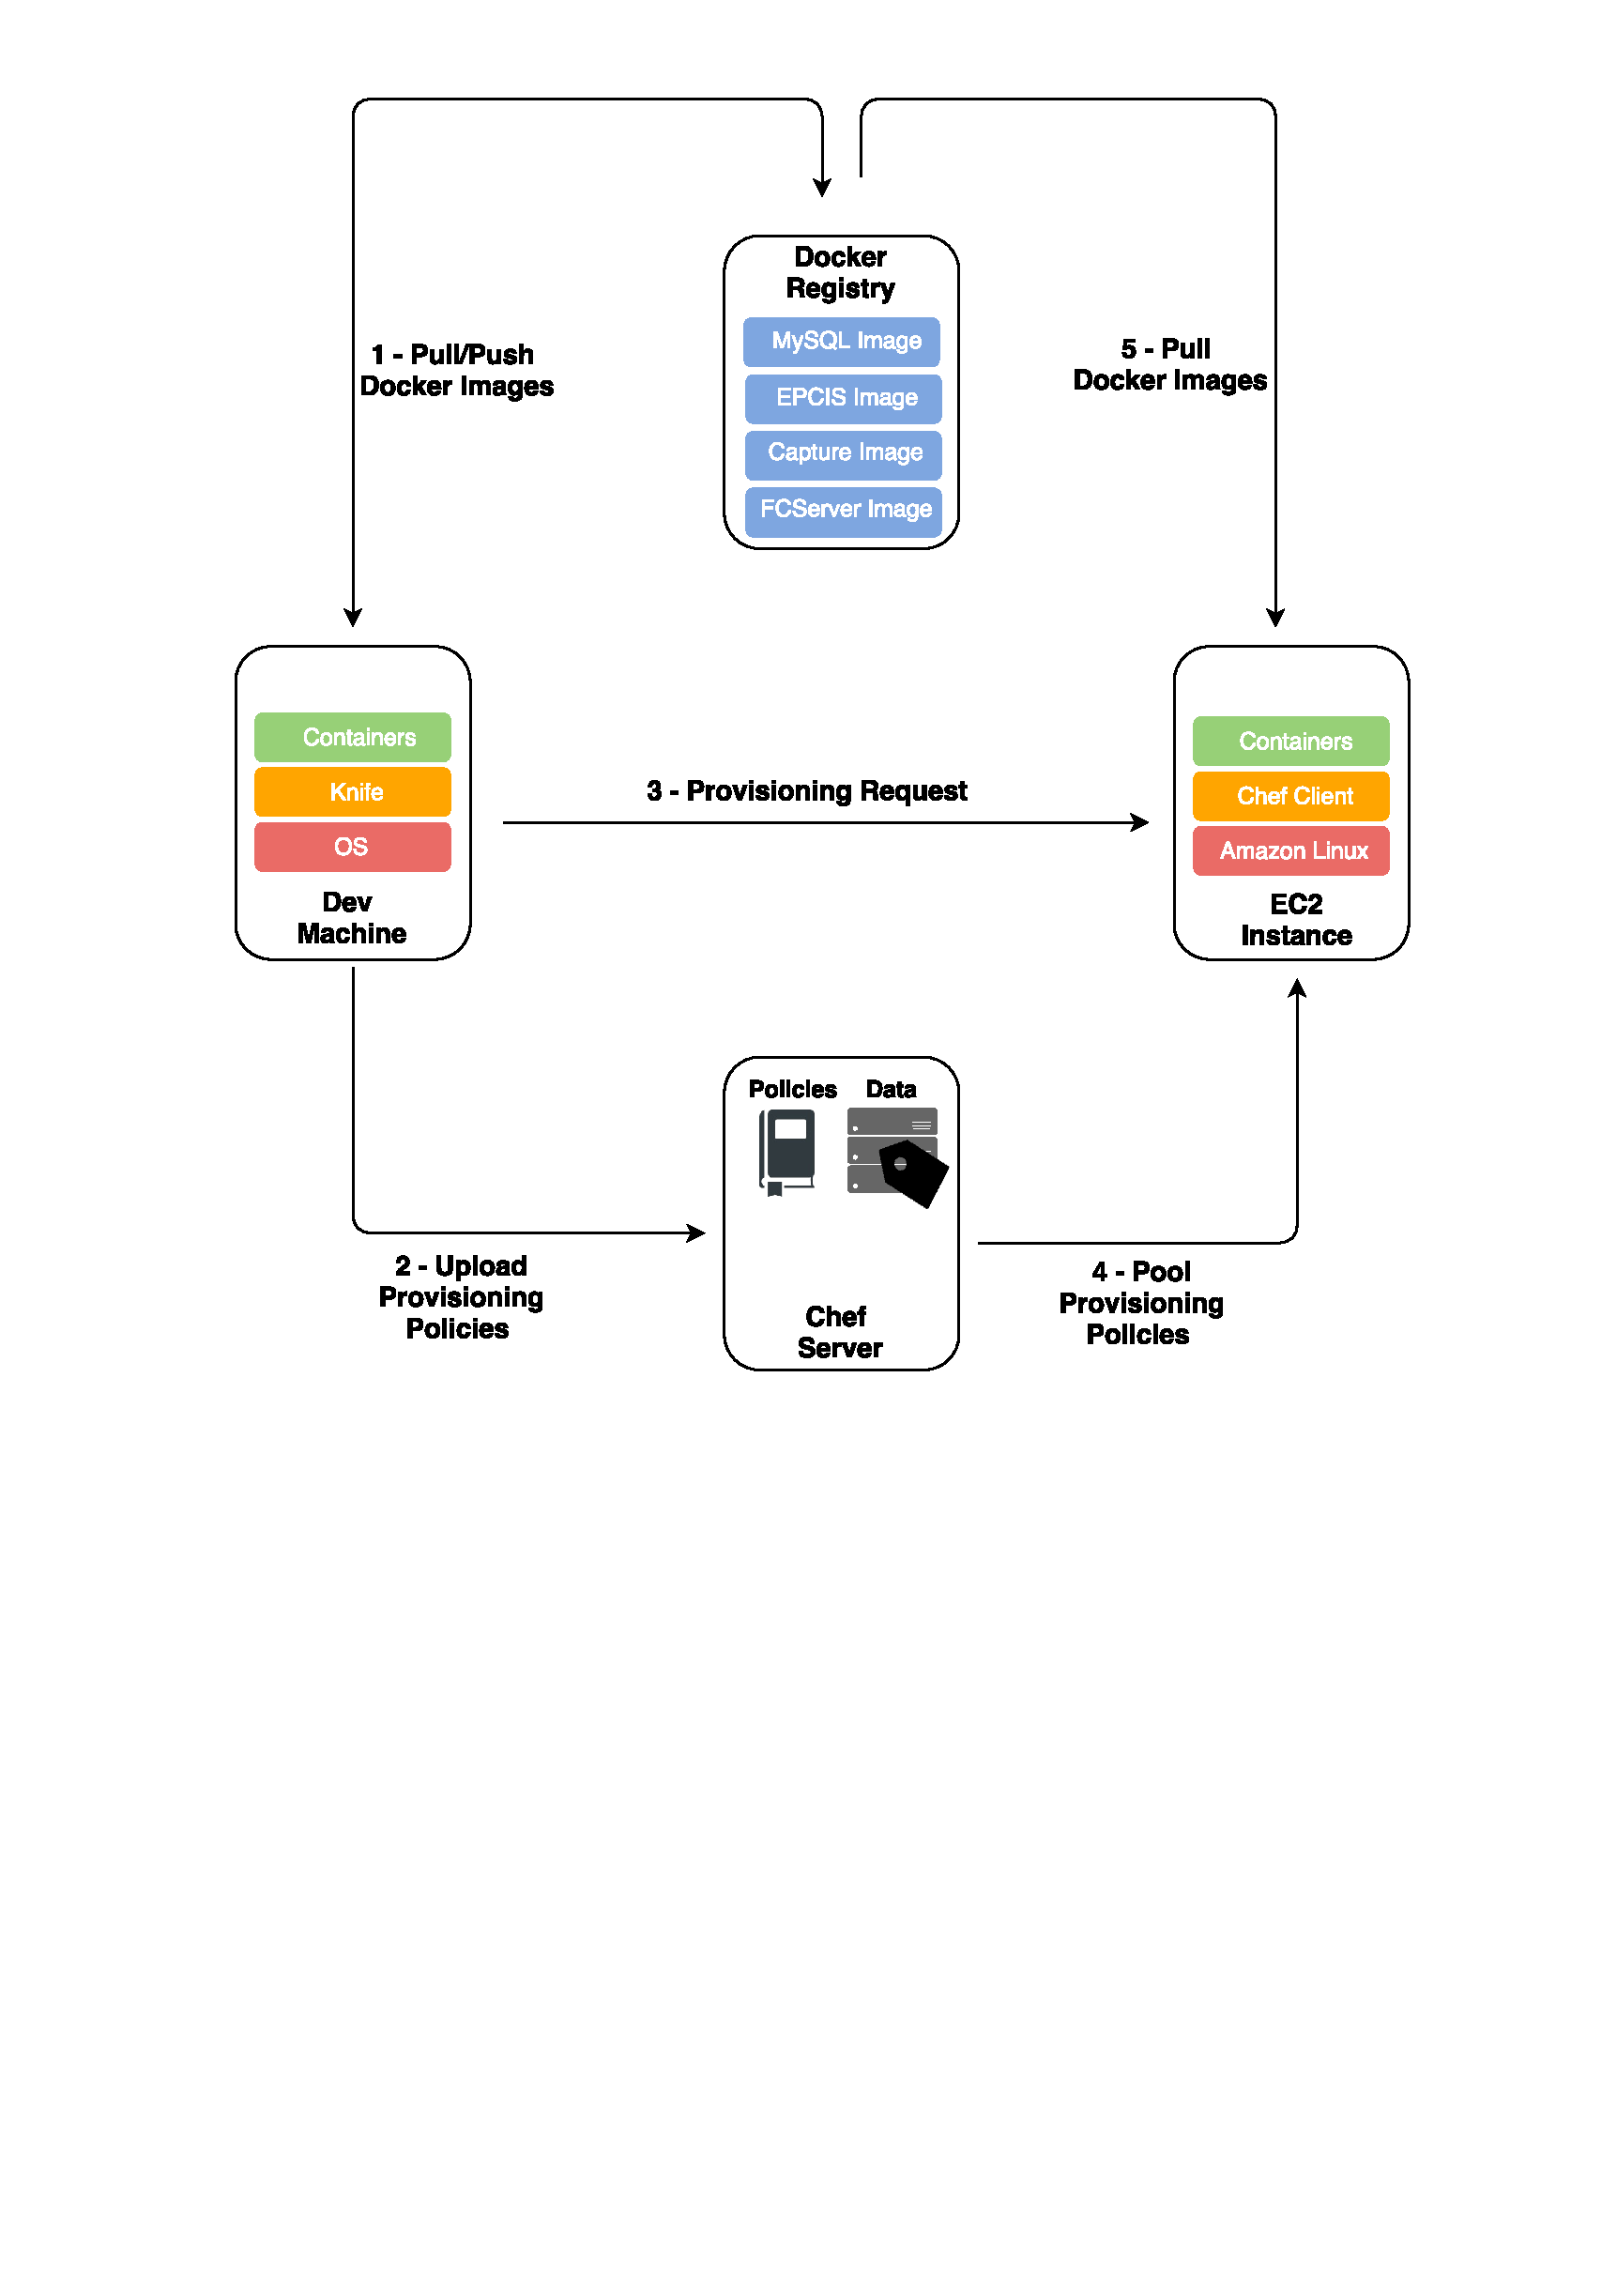
\includegraphics[width=.8\textwidth]{./images/c4t-tech-architecture}}%
\caption[Automatic provisioning workflow.]{Automatic provisioning workflow.}
\label{fig:provisioning_tech_architecture}
\end{figure}

In a development environment the Docker images are built and then uploaded to the Docker Registry
repository (1). The provisioning of the cloud resources is described in the cookbooks that are uploaded
to the Chef server (2). The provisioning request (3) is performed using \textit{knife}, that allows to
describe the image type, the instance type and the policies - e.g. the \textit{role(s)} and/or \textit{recipe(s)} -
that need to be applied on each provisioned node. Then the Chef client runs the configuration policies
that are pulled from the Chef server (4). In our solution the Chef client apply the configuration recipes
that are described in the role assigned to the node. The Chef client pulls the Docker images from the
remote repository, build the containers based on those images and finally applies the configuration
that is associated to each container.\\

We decide to chose Chef instead of its competitors - i.e. Puppet and Ansible - for several
reasons, where the main one is \textit{knife}. Knife tool is very powerful and allow us to
interact with our entire infrastructure. For instance, it is possible to bootstrap a new server,
apply a role to a set of nodes in our environment. Furthermore, with \textit{knife ssh} it is possible
to execute a command on a certain number of nodes in our environment. For instance, if we change
the role configuration that is assigned to a set of nodes in our infrastructure, knife allows to
update all these nodes with the most recent policy with a single command.\\

Also, knife provides plugins for several cloud providers, such as \gls{AWS}\footnote{\url{https://aws.amazon.com/}},
and Google Compute Engine\footnote{\url{https://cloud.google.com/compute/}}. These plugins allow
the provisioning of the application in the cloud providers infrastructure using the same resources - e.g.
roles, recipes, etc - for all available providers.

% Docker containers
\subsubsection{Docker Containers}
\label{subs:impl_docker}
Docker containers are used to provisioning the software stack of Fosstrak platform. A complete
installation of Fosstrak requires a compatible Java \gls{SDK}, a full MySQL database and a Apache Tomcat
server.\\

We are provisioning a single container for each component of Fosstrak, the \gls{EPCIS} repository,
the Capture application, the \gls{FCServer} and also for the MySQL database, As illustrated in Figure~\ref{fig:impl_containers}.
In our implementation, the container images of Fosstrak are published in the Docker Hub repository
to later be used to create the containers.\\

% Container stack
\begin{figure}[!ht]
\centering
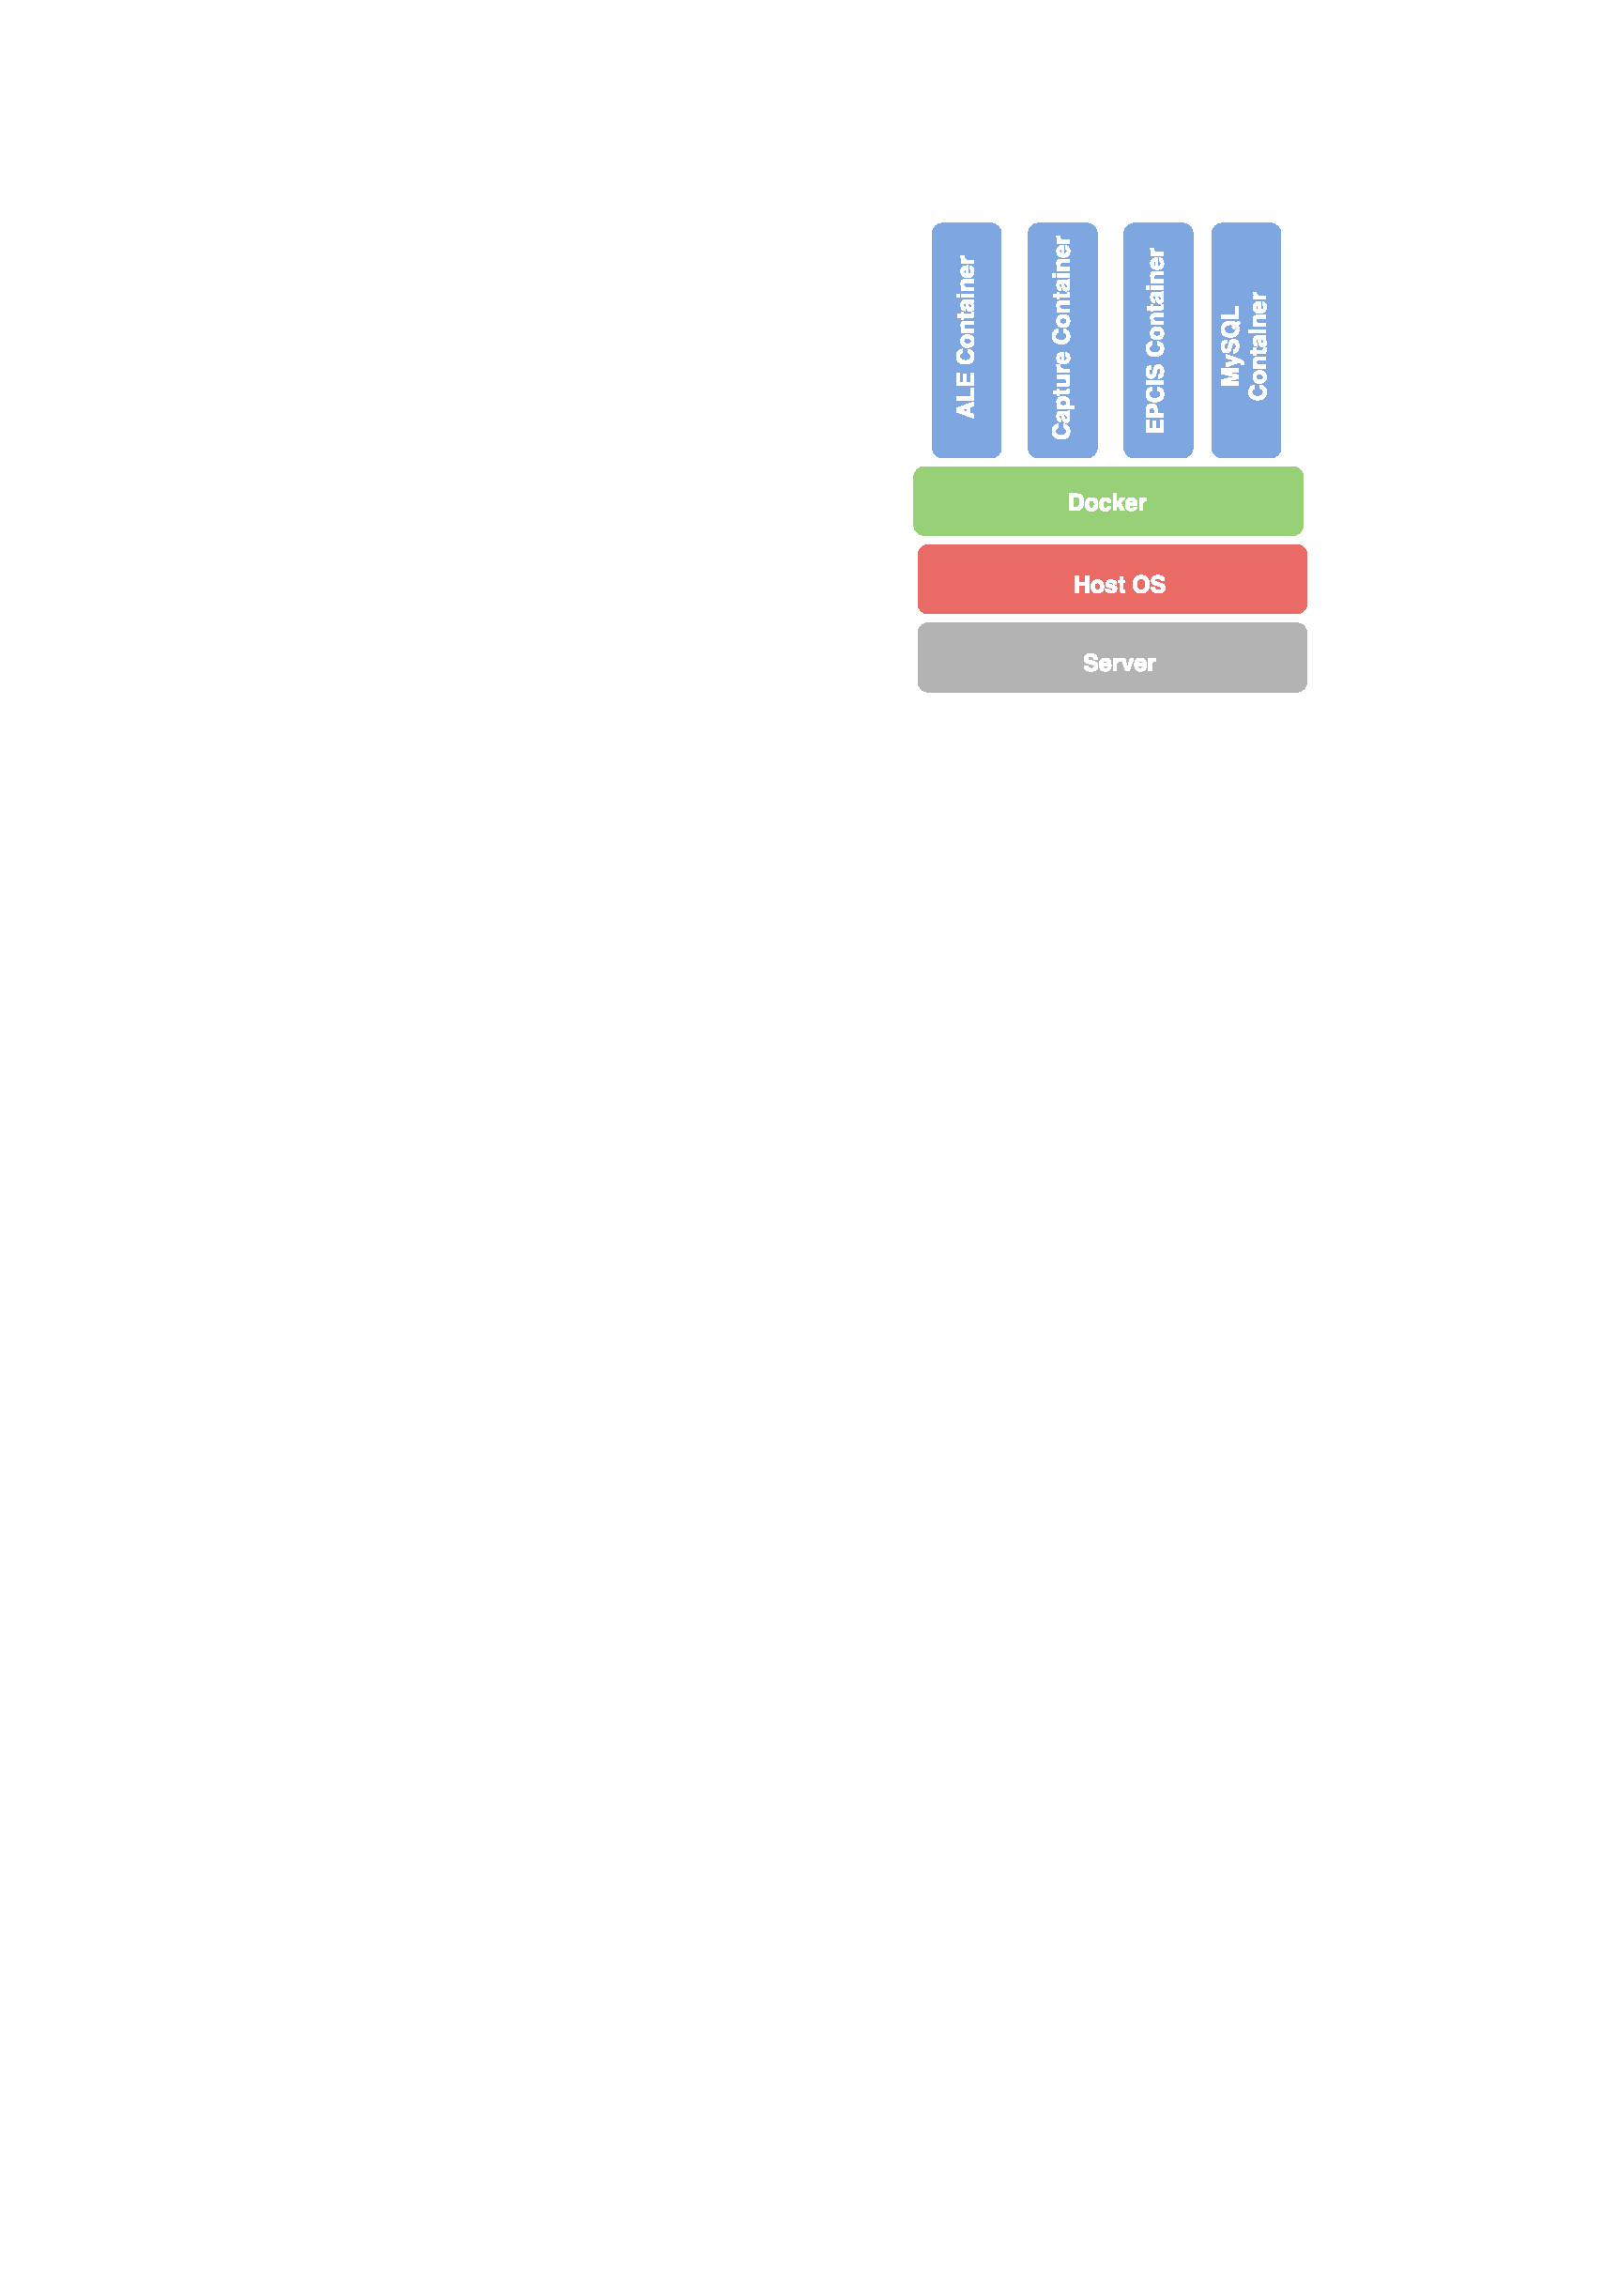
\includegraphics[width=.3\textwidth]{./images/docker-stack}
\caption[Fosstrak containers stack.]{Fosstrak containers stack.}
\label{fig:impl_containers}
\end{figure}

By default each container runs a process that is isolated from the other processes that shares the same
environment (kernel). Compared with the isolation provided by traditional \glspl{VM} - which are fully
isolated - the isolation provided by Docker containers is less secure, since that if a container has
its security broken, it is possible that other containers and host may be compromised.\\

In order to connect the different modules of the Fosstrak, our containers are
linked through the \textit{linking system} provided by Docker. This mechanism creates a secure tunnel
between the containers, allowing the recipient container to access selected data about the source container.
For instance, our \gls{EPCIS} container - which is linked to the MySQL database container - is able to
access information about the MySQL container.\\

The reasons that we chose Docker containers instead of traditional \glspl{VM} is that containers
require less disk space and read/write (I/O) operations in the disk when compared with traditional
\gls{VM} images \cite{merkel2014docker}. Furthermore, Docker containers are easier to port to another
infrastructure when compared with traditional \glspl{VM} because when a container requires that the
application and all of its dependencies are ported together while the \glspl{VM} require that the
entire application, the guest operating system, the binaries and libraries are ported, which can be
several \glspl{GB} in size.

% Smart Warehouse Deployment
\section{Smart Warehouse Deployment}
\label{sec:sol_smart_warehouse_deployment}
Our smart place is an automated warehouse where automated vehicles transport tagged objects that can
be identified by readers and sensors that are deployed in the place, as described in Section~\ref{sub:domain}.
In traditional solutions, the application is provisioned in a local infrastructure. Although such
approach guarantees that the low-latency requirements are meet, this solution comes with several
downsides - such as the low scalability, infrastructure and maintenance costs - that can be a barrier
for these applications.\\

Leveraging the infrastructure required to provisioning the smart place applications to the cloud
guarantees that the bottlenecks of traditional solutions are solved. However, we also need to
guarantee that the latency requirements of these applications are fulfilled. The cloud and fog concepts
give us more flexibility to perform the deployment of smart place applications, which allow us to
provisioning the application modules in a more distributed way. The following sections describe
the deployment approaches of smart place applications based in the cloud and fog.

% Cloud approach
\subsection{Cloud Deployment}
\label{sub:sol_cloud}

% Cloud approach
\begin{figure}[ht!]
\centering
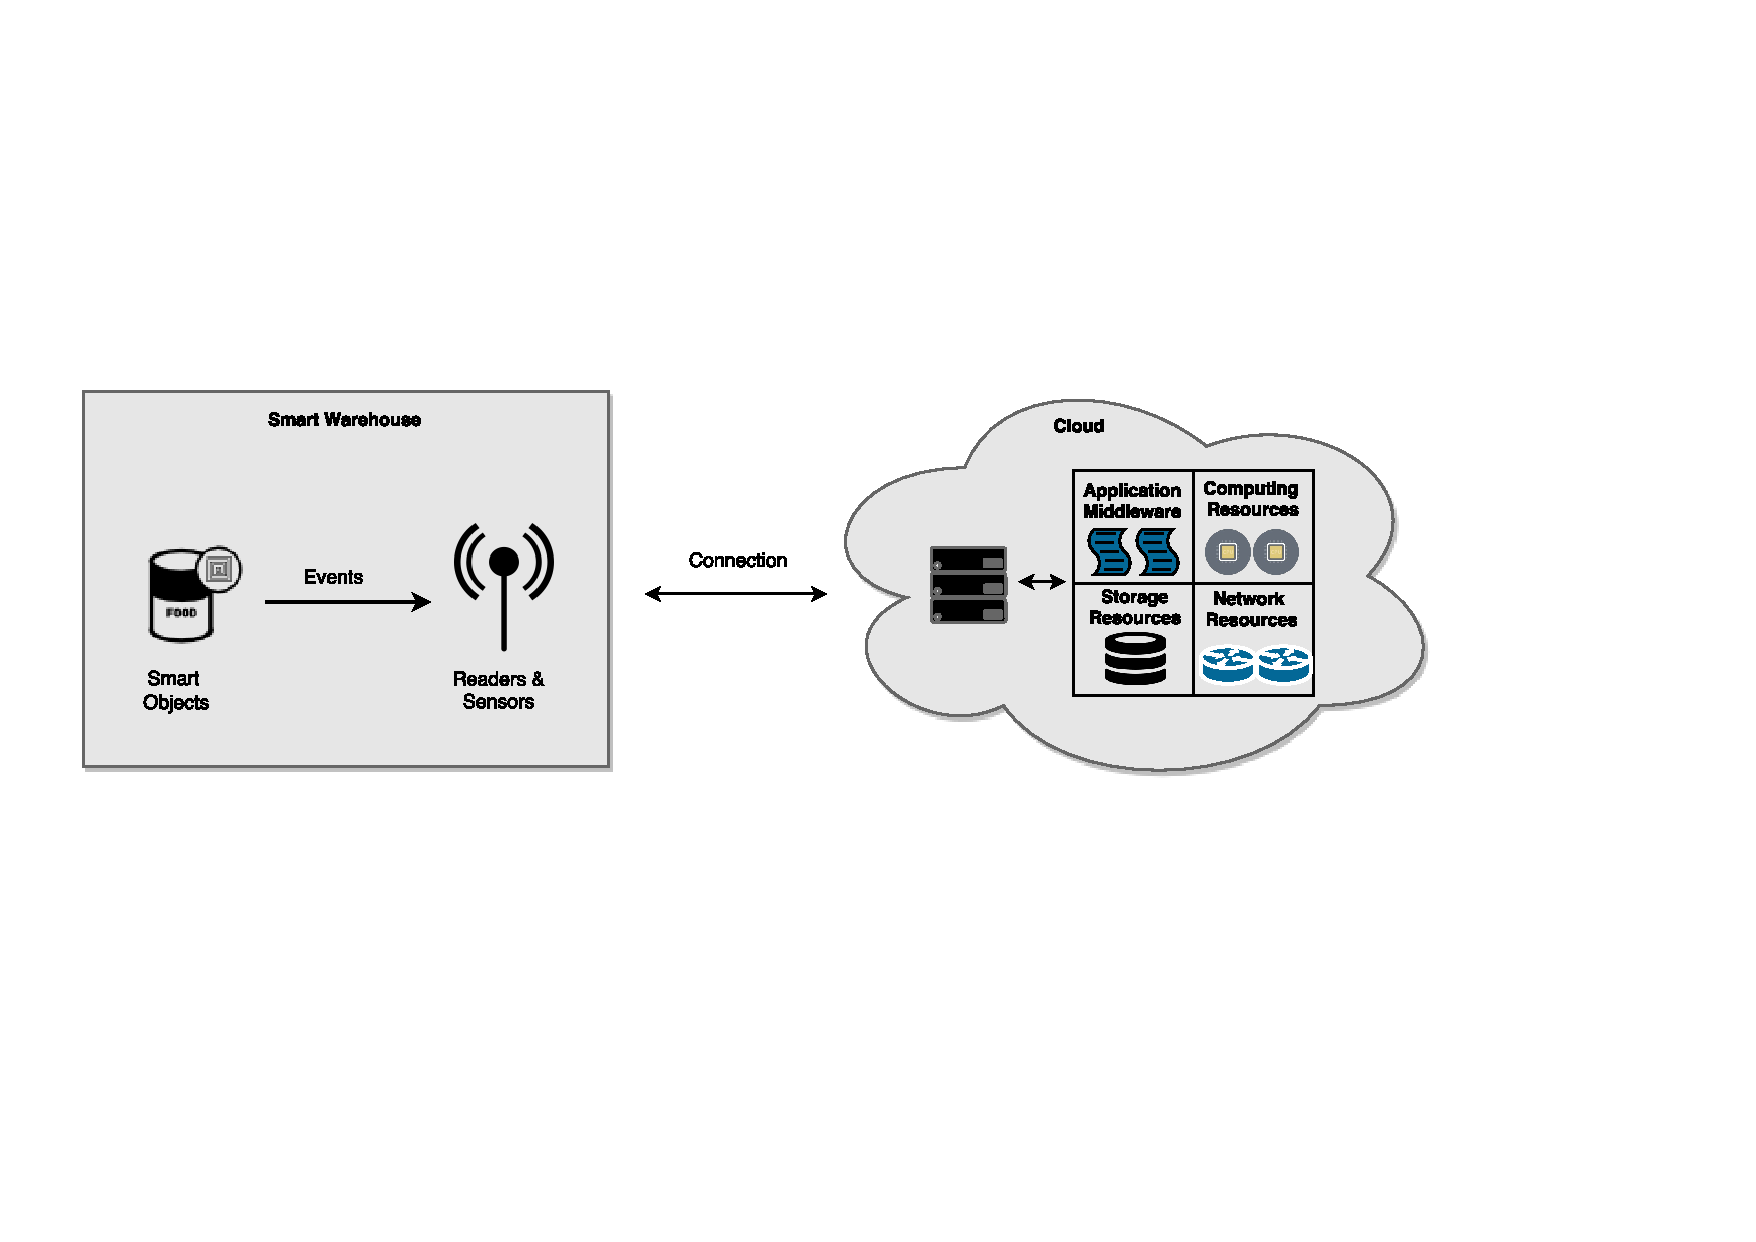
\includegraphics[width=\textwidth]{./images/solution_cloud_architecture}
\caption[Cloud-approach: conceptual architecture.]{Cloud-approach: smart warehouse conceptual architecture.}
\label{fig:solution_cloud_architecture}
\end{figure}

Figure~\ref{fig:solution_cloud_architecture} presents the architecture of a cloud-based smart warehouse.
The warehouse is composed of smart objects, sensors and readers that capture the events that occurs
in the warehouse. The application middleware is provisioned in the cloud, which virtualizes the computing,
storage and network resources needed to support the application.\\

The smart warehouse can be connected to the cloud through a physical or wireless connection.

% Fog approach
\subsection{Fog Deployment}
\label{sub:sol_fog}

% Fog approach
\begin{figure}[ht!]
\centering
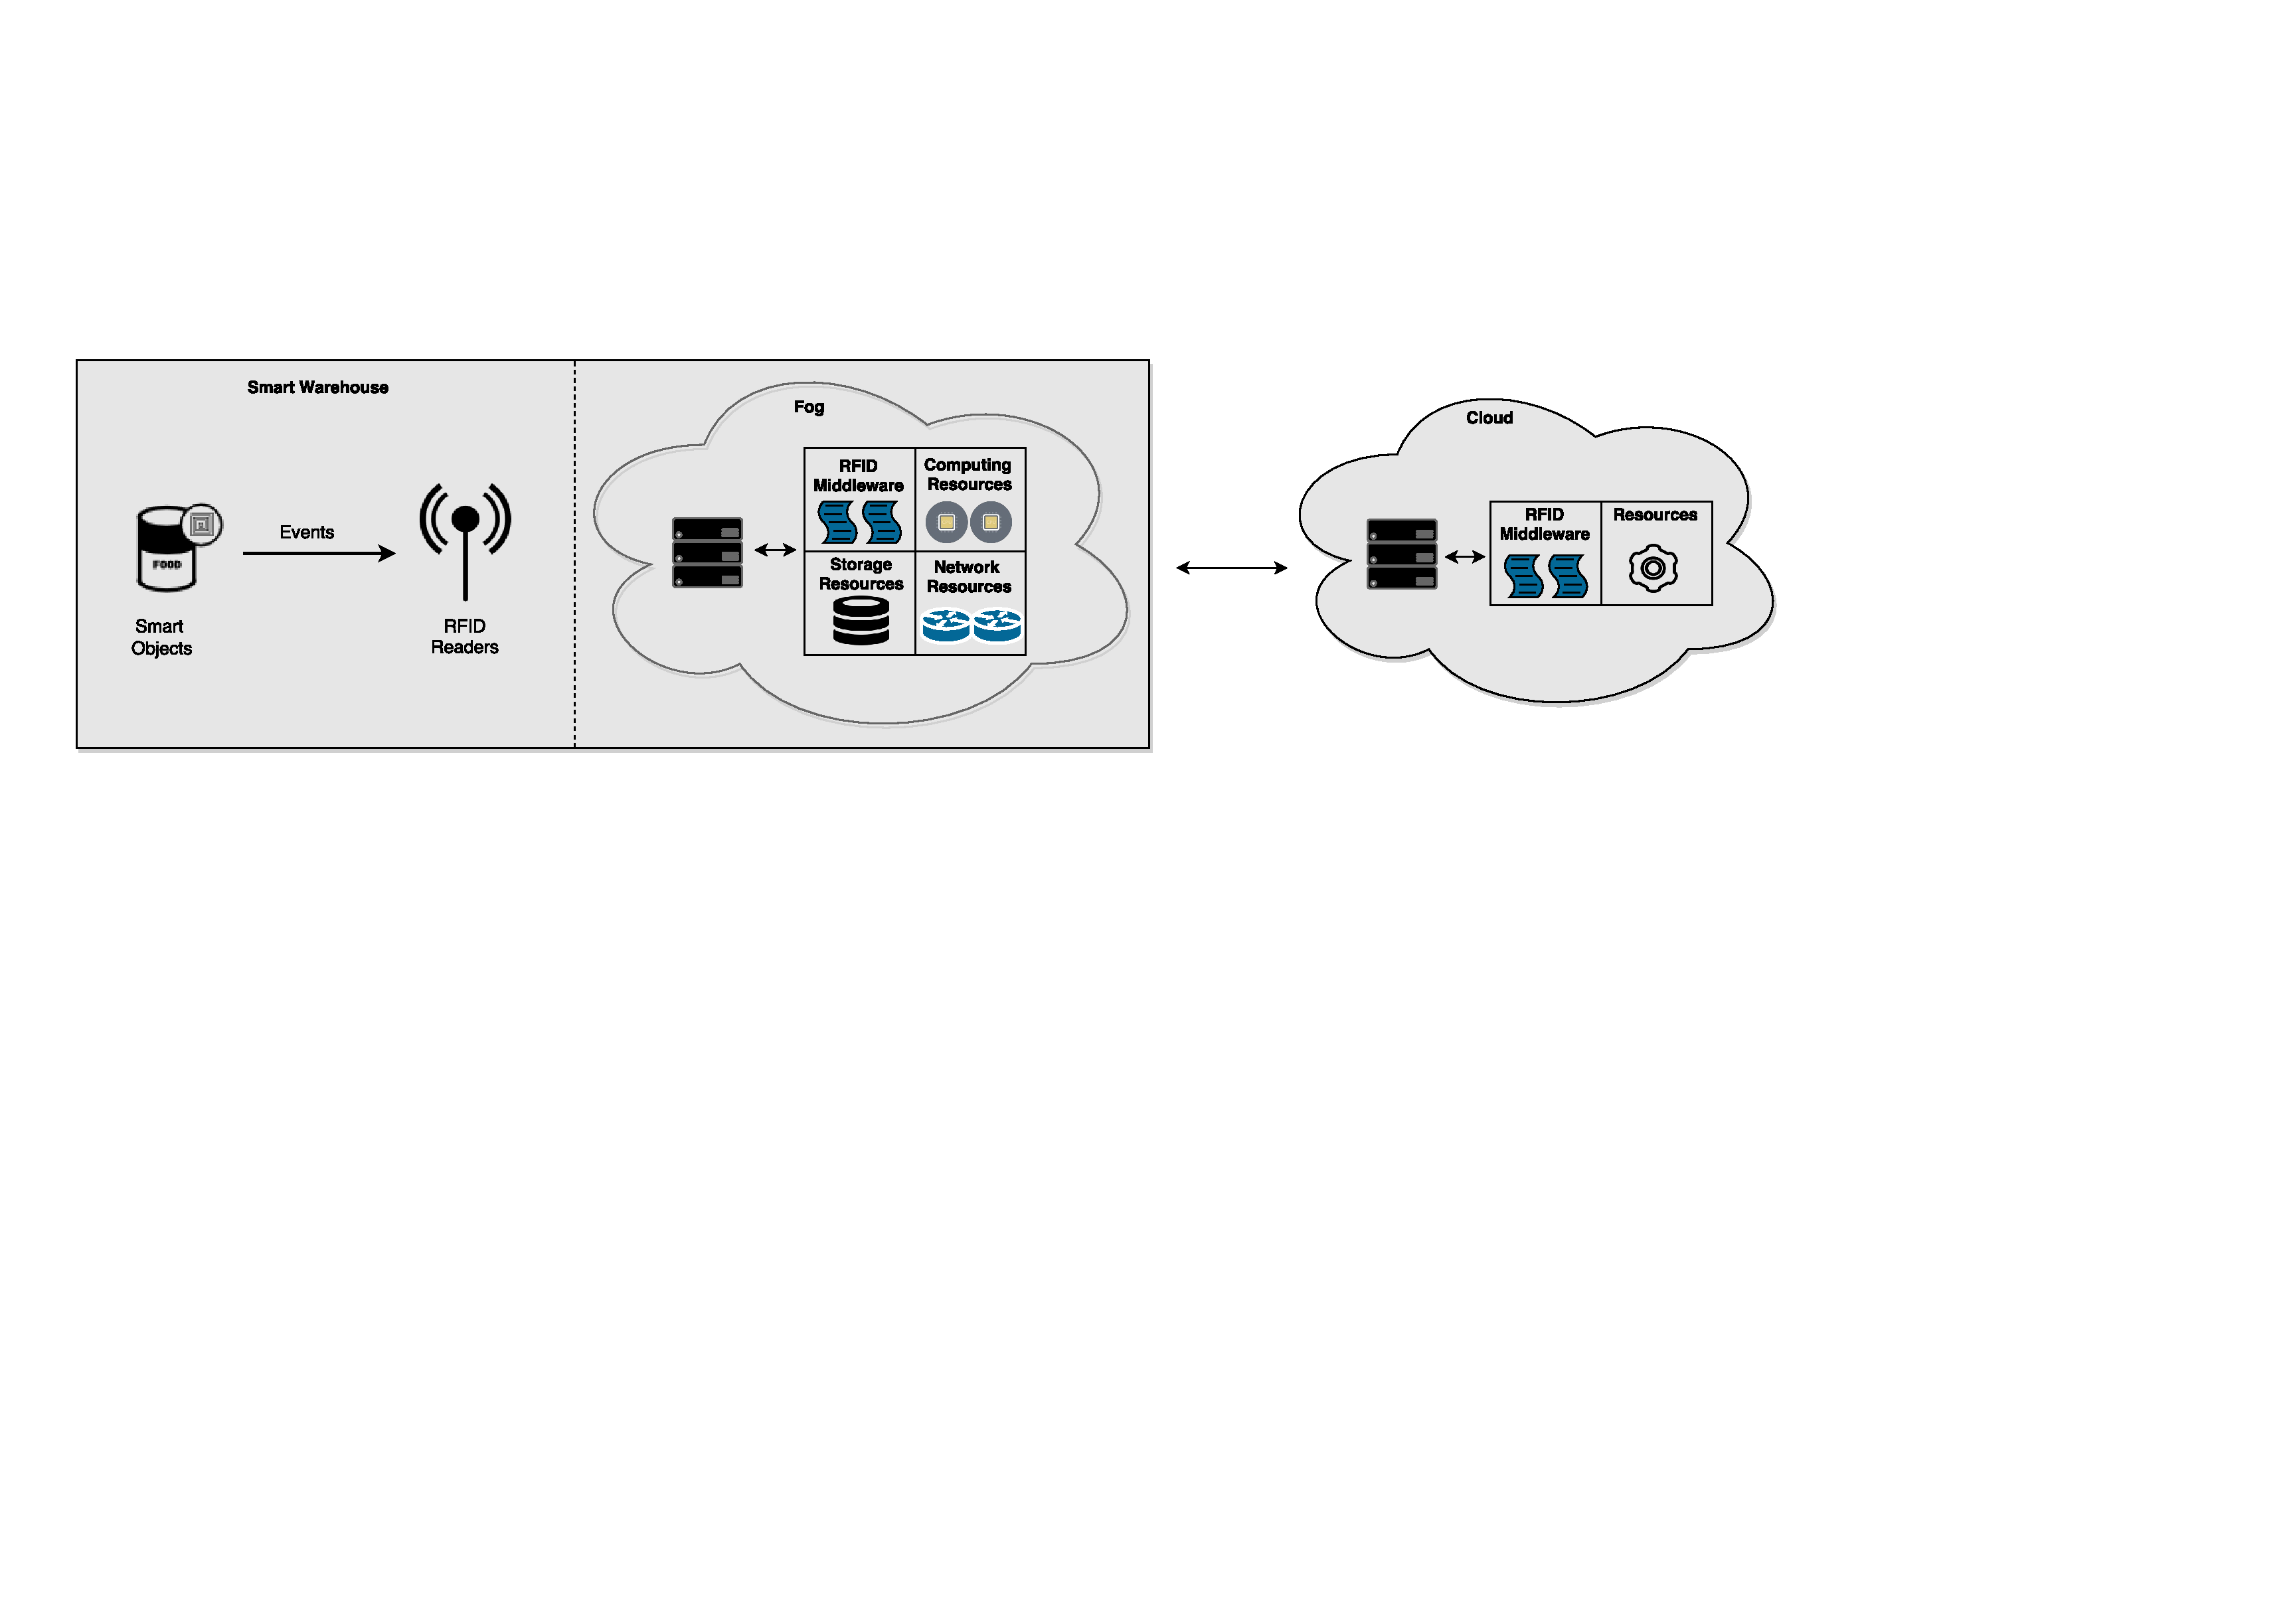
\includegraphics[width=\textwidth]{./images/solution_fog_architecture}
\caption[Fog-approach: conceptual architecture.]{Fog-approach: smart warehouse conceptual architecture.}
\label{fig:solution_fog_architecture}
\end{figure}

Figure~\ref{fig:solution_fog_architecture} presents the architecture of a fog-based smart warehouse.
As in the cloud-based approach the warehouse is composed of smart objects, sensors and readers.
The proposed approach aims to extend the cloud paradigm to the edge of the network. The fog achieves
that by virtualizing computing, storage and network resources. Unlike the cloud infrastructure, that
usually is provisioned thousands of kilometers from the smart warehouse, the fog infrastructure
usually is provisioned closest to the smart warehouse network.\\

Regarding the application middleware, the application components are distributed across the cloud and
fog. The components responsible for storing the data during a long period of time are provisioned in
the cloud. The components responsible for performing real-time processing of the data generated in the
warehouse, and the components that filter the data that is consumed locally and must be delivered to
the cloud are provisioned in the fog.\\

Both the smart warehouse as the fog can be connected respectively to the fog and cloud through
several types of connection, from a physical connection to a wireless connection.

\subsection{Implementation Details}
\label{sub:implementation}
The smart warehouse setup was based in a demonstration scenario described by Correia et al. \cite{correiaalpharfid},
as illustrated in Figure~\ref{fig:rfidapp_setup}.\\

% RFID application setup
\begin{figure}[ht!]
\centering
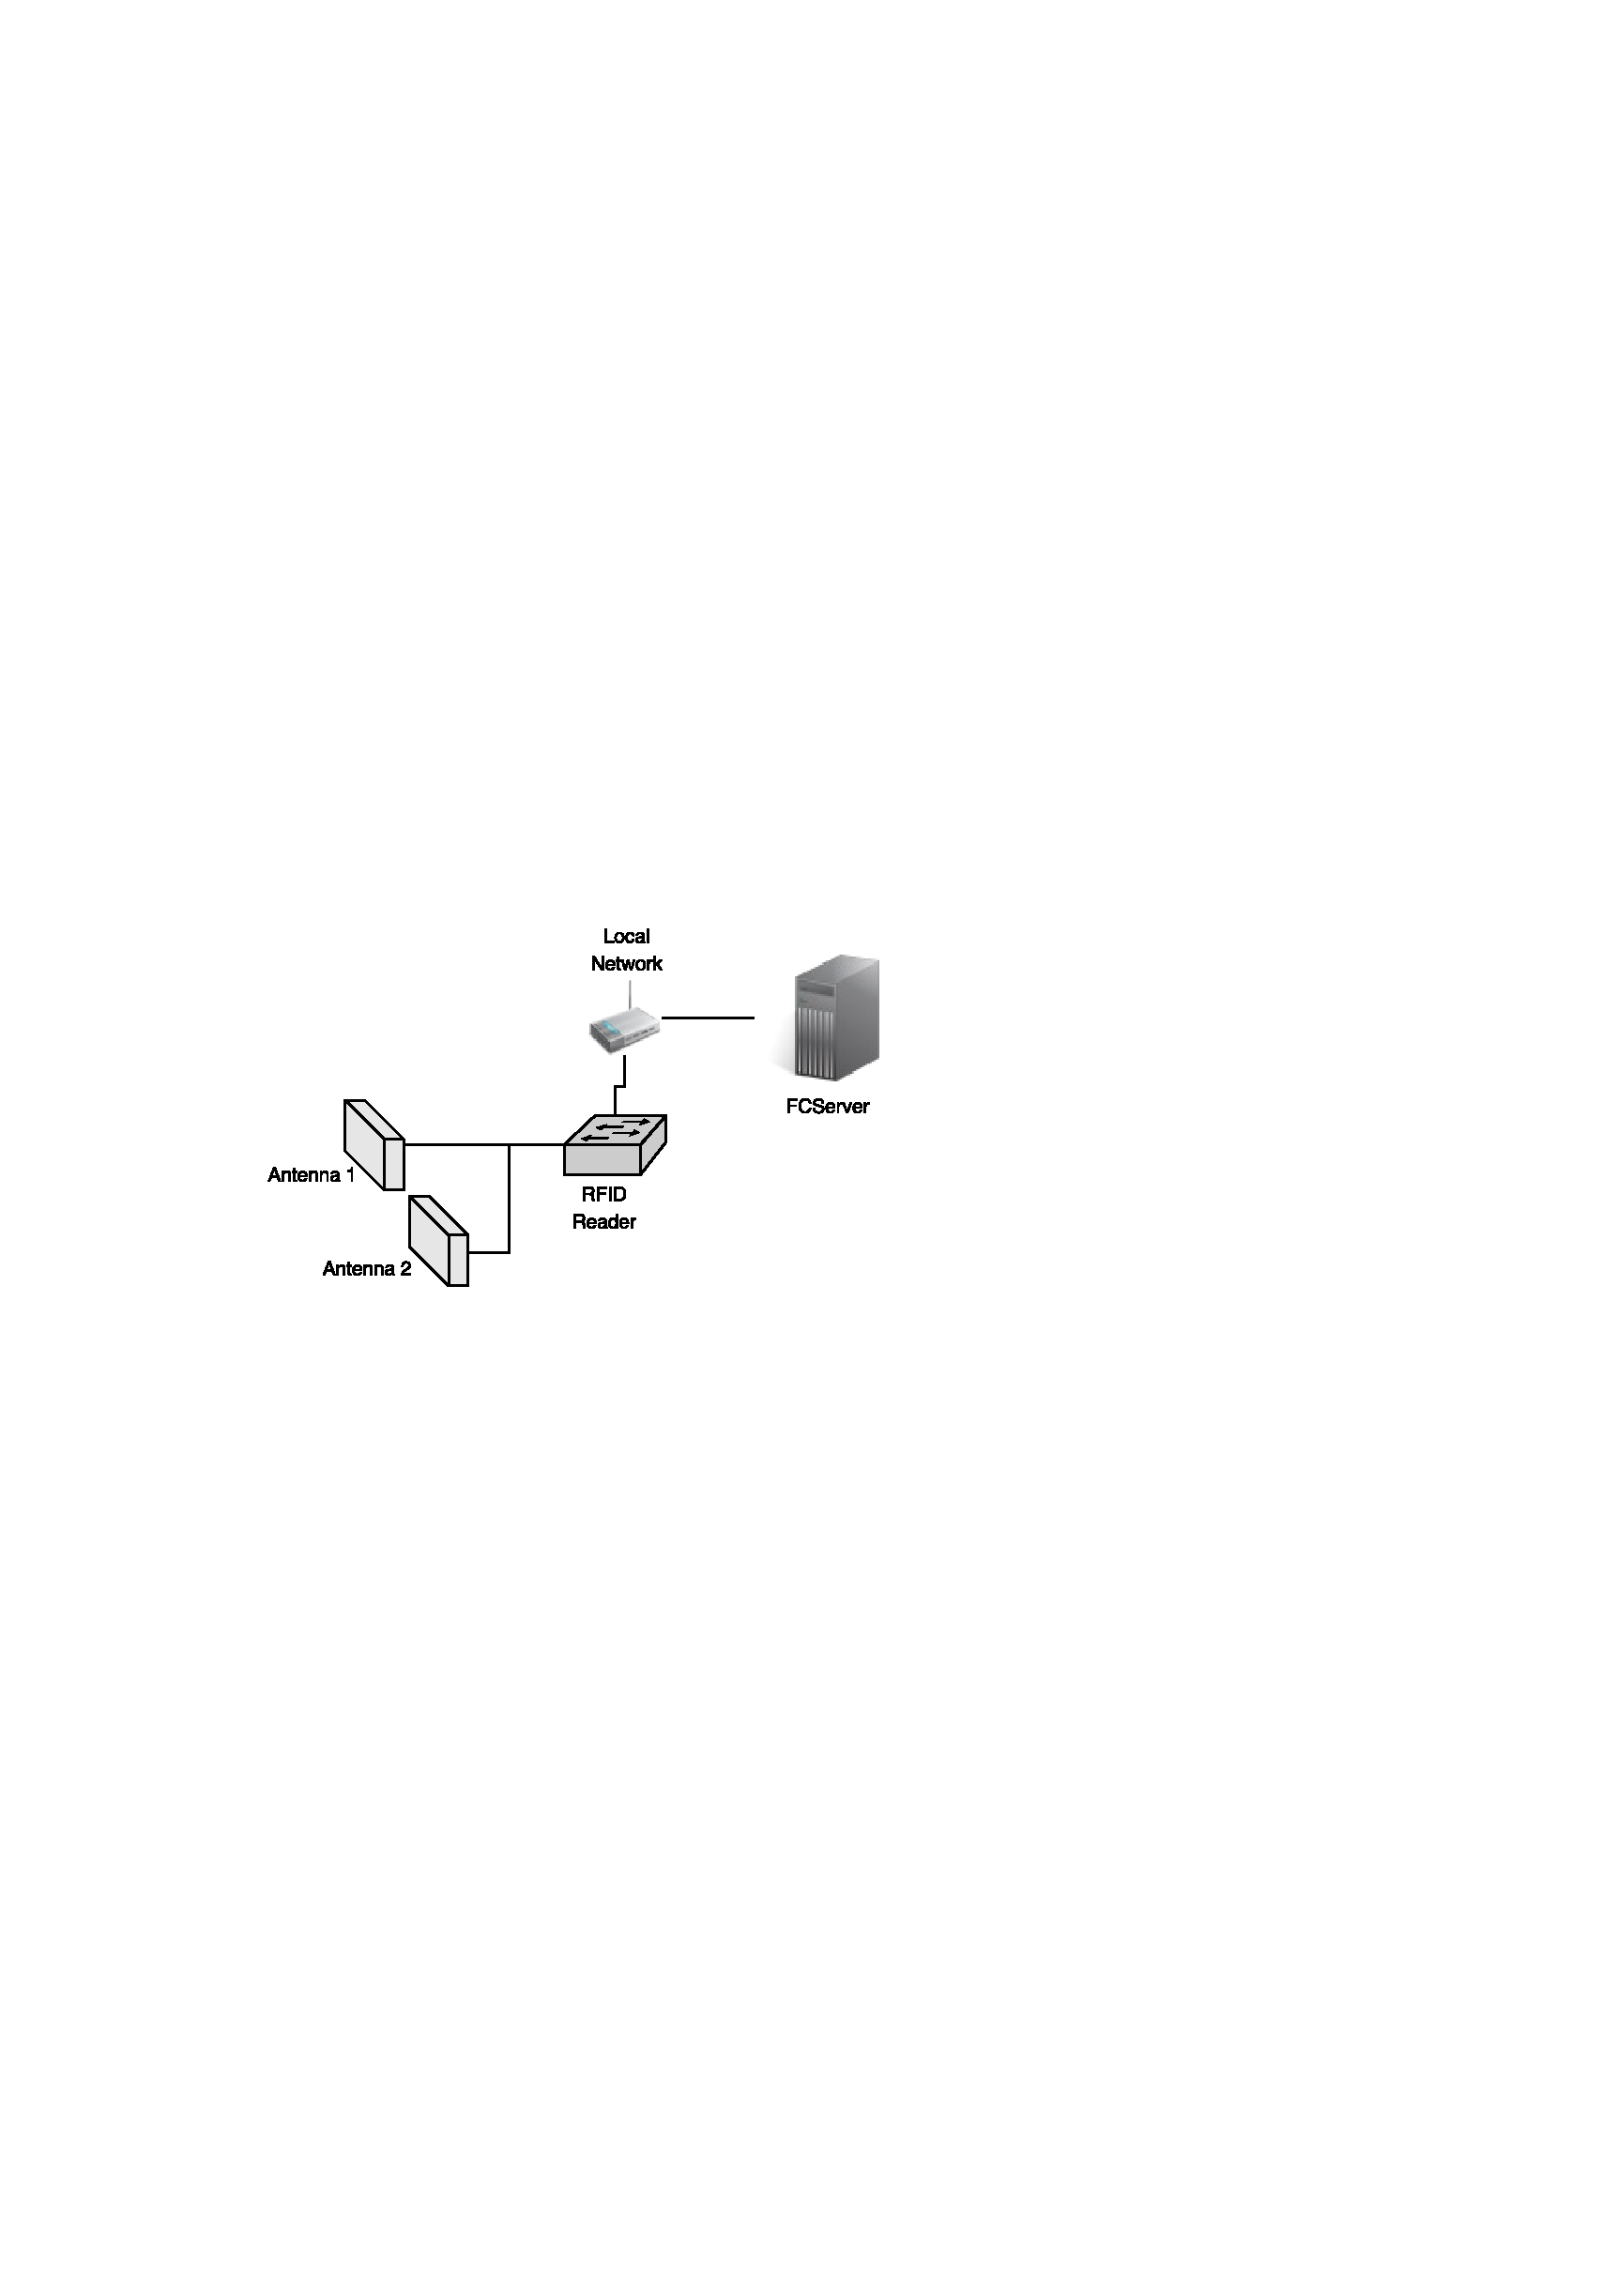
\includegraphics[width=.6\textwidth]{./images/rfidapp_setup}
\caption[RFID application setup.]{RFID application setup.}
\label{fig:rfidapp_setup}
\end{figure}

The warehouse is composed of a robot transporting tagged products that are identified by \gls{RFID} readers
deployed in the physical space. To monitor the robot inside the warehouse, the Fosstrak \gls{RFID} middleware
is used. In our implementation, the \gls{RFID} readers are emulated through the Rifidi Emulator, which uses
the \gls{LLRP} protocol to communicate with the Fosstrak platform.

% Cloud approach
\subsubsection{Cloud Deployment}
\label{subs:imp_smart_warehouse_cloud}

% Cloud approach
\begin{figure}[ht!]
\centering
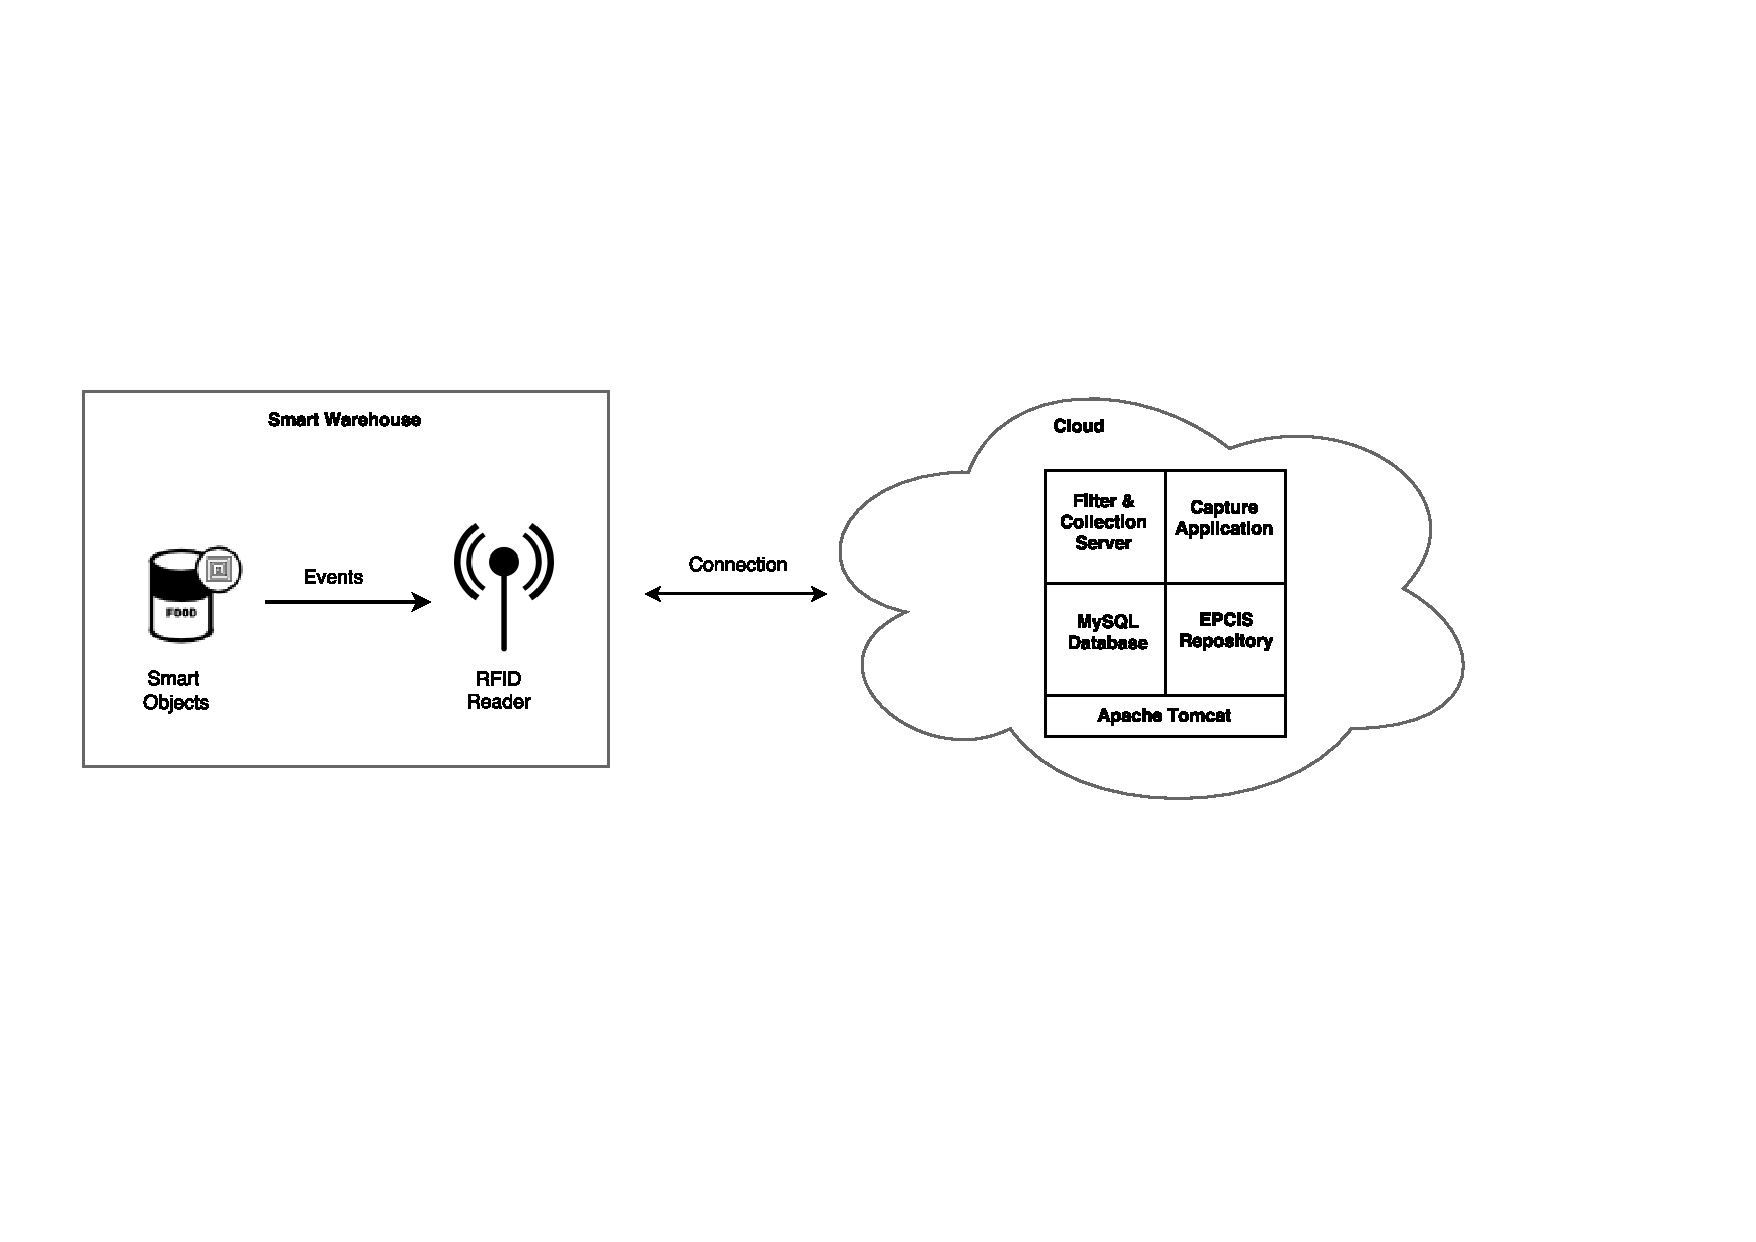
\includegraphics[width=\textwidth]{./images/implementation_cloud_architecture}
\caption[Cloud-approach: technological architecture.]{Cloud-approach: smart warehouse technological architecture.}
\label{fig:implementation_cloud_architecture}
\end{figure}

The \gls{RFID} middleware is provisioned in the cloud in a single virtual machine. In the
Fosstrak implementation the \gls{FCServer}, \gls{EPCIS} repository and the Capture application
requires an Apache servlet container to deploy and run the web applications. The \gls{EPCIS}
repository is connected to a MySQL database that stores the event data. The technological architecture
for the cloud approach is presented in Figure~\ref{fig:implementation_cloud_architecture}.\\

The smart warehouse can be connected to the cloud through a physical (e.g. \gls{ADSL} or Fiber-optic)
to a wireless connection (e.g. Wi-Fi, 3G or \gls{LTE}).

% Fog approach
\subsubsection{Fog Deployment}
\label{subs:imp_smart_warehouse_fog}

% Fog approach
\begin{figure}[ht!]
\centering
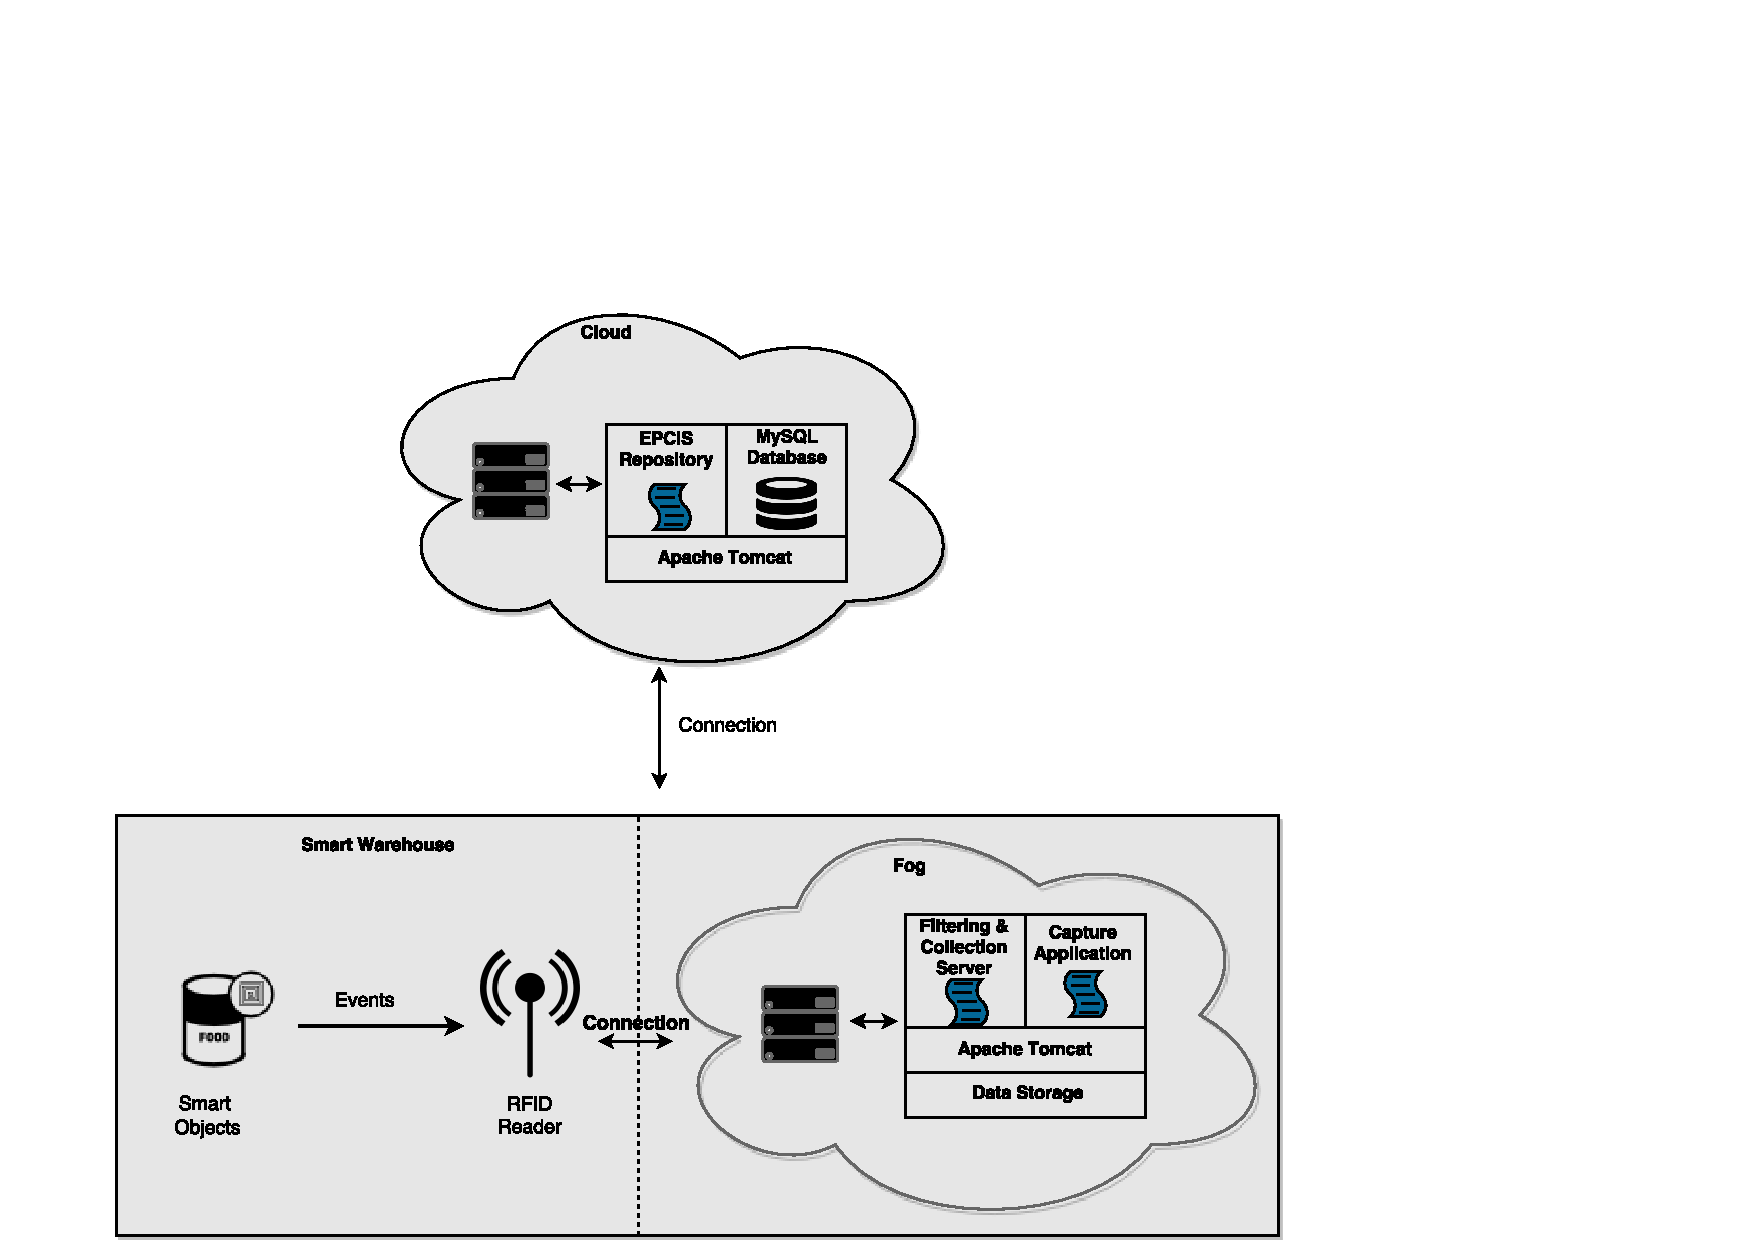
\includegraphics[width=\textwidth]{./images/implementation_fog_architecture}
\caption[Fog-approach: technological architecture.]{Fog-approach: smart warehouse technological architecture.}
\label{fig:implementation_fog_architecture}
\end{figure}

The \gls{RFID} middleware is provisioned across the fog and the cloud. At the cloud,
all the software components are provisioned in a single \gls{VM}. The \gls{EPCIS} repository is deployed
and running on top of an Apache Tomcat servlet instance. The repository is connected to a MySQL
database, which stores the event data. In the current implementation the fog was built with a traditional
\gls{VM}. The \gls{FCServer} and the Capture application are deployed and running on top of a single
Tomcat servlet instance. The Capture application sent the events collected by the \gls{FCServer} to
the \gls{EPCIS} repository through the \textit{\gls{EPCIS} Capture Interface} - via \gls{HTTP} requests.
Figure~\ref{fig:implementation_fog_architecture} presents the technological architecture for the fog
approach.\\

Both the smart warehouse as the fog can be connected respectively to the fog and cloud through several
types of connection, from a physical connection (e.g. \gls{ADSL} or Fiber-optic) to a wireless connection
(e.g. Wi-Fi, 3G or \gls{LTE}).

% Summary
\section{Summary}
\label{sec:sol_summary}
In this chapter we proposed a solution to automate the provisioning of smart warehouse applications
based on the \gls{RFID} technology in the cloud. The implementation details for the proposed
solution and the technological components used in our implementation also were discussed.\\

Our provisioning mechanism is based on the Chef tool. To provisioning Fosstrak's software stack we are
using Docker containers in alternative to the traditional \glspl{VM}. The provisioning mechanism relies
on the \textit{recipes}, \textit{roles} and the \textit{knife} command, which are provided by Chef.
We defined a set of recipes that allow to describing how the Fosstrak software stack should be installed
in a node while the roles allow to attributing responsibilities to a specific node. The knife command
is used to execute the provisioning request and to interact with the provisioned infrastructure.\\

The provisioning mechanism implemented in this work allows to perform the deployment of a smart place
application based in Fosstrak across the cloud and fog, although it can be extended to support other
\gls{RFID} middleware platforms. The flexibility in the deployment provided by the cloud and fog
concepts will allow us to evaluate the approaches and chose which one is more adequate to support smart
place applications based on the \gls{RFID} technology.
